\Chapter{A fejlesztőkörnyezet implementációja}

\graphicspath{{./kepek/}}

\Section{Minimális program: egy fáljt kezelő kódszerkesztő}

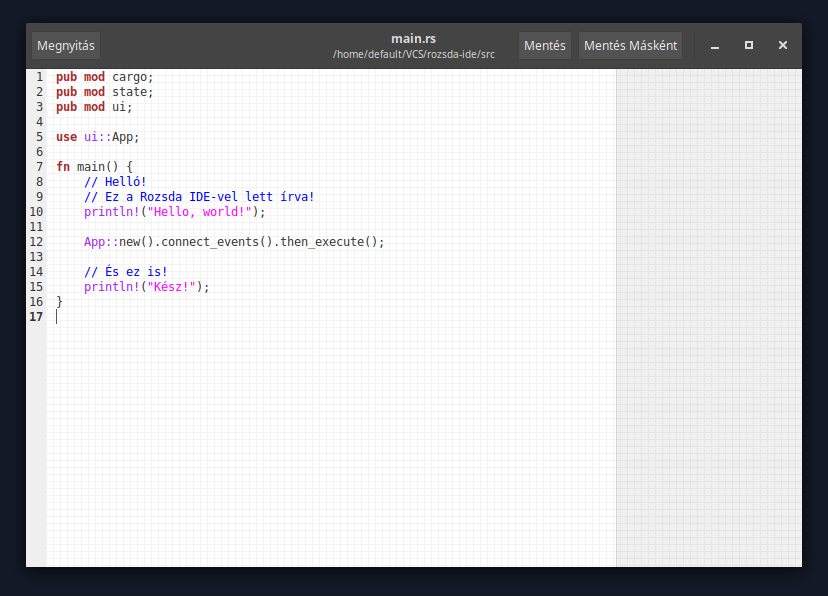
\includegraphics[width=\textwidth]{program-mvp}

A program implementációját egy olyan minimális életképes termék elkészítésével kezdjük,
ami meg tud nyitni egyszerre egy fájlt, annak tartalmát megfelelően dekorálja,
ha az egy Rust forráskód-fájl, és tud az eredeti, vagy egy másik megadott fájlba menteni.

A programnak ez a része Michael Murphy \textit{Simple Common Mark Editor} projektjén alapul.\cite{gtk_tutorial}
Murphy programra Markdown formátumú fájlokat kezel, illetve azokat HTML formátumra lefordítja,
és megjeleníti a felhasználónak.
A leglényegesebb változtatások ezen a programon a Markdown nyelv lecserélése a Rust nyelvre,
a projekt frissítése egyrészt a Rust 2018-as verziójára, illetve a függőségek frissítése a legújabb verziókra.

A projekt egy \texttt{cargo new} parancshívással kezdődik.

\SubSection{Cargo.TOML}

\lstinputlisting{./kodreszletek/01_cargo.toml}

A projekt Cargo.TOML-jában nincs semmi különös.
A \texttt{package} kategória legtöbb értéke nem lényeges, mivel ezeket a Cargo használja fel
a \url{crates.io}-ra való publikáláskor.
A mi szempontunkból az egyetlen kitűnő érték az az \texttt{edition}, amivel a Rust 2018-as
kiadásának használatát kérjük a \texttt{rustc}-től.
A 2015-ös és a 2018-as kiadás kompatibilis egymással,\cite{rust:editions}
a legnagyobb előnye a frissítésnek a programozás megkönnyítése az új nyelvi tulajdonságokkal.
A \texttt{dependencies} kategória leírja a projekt függőségeit, és a függőségek kötelező verziószámát.
Itt konkrét verziószámokat adtunk meg, de lehetőség van a Cargo-ra hagyni az optimális verziók kiderítését is.
A \texttt{GTK} és a \texttt{SourceView} esetén azt is megadjuk, 
hogy ezek a Rust könyvtárak az alattuk lévő könyvtárak melyik verziójára épüljenek rá
(a megadott \texttt{SourceView} Rust könyvtár verziószáma disztinkt a C-ben íródott \texttt{SourceView}
projekt verziószámától).

\SubSection{Az \texttt{App} és a \texttt{SourceView}}

A felhasználói felülettel kapcsolatos forráskódokat az olvashatóság kedvéért egy modulba tesszük,
az \texttt{ui} modulba.
A modulkészítés a Rust 2018-as kiadásában forrásfájlokon alapul -- 
minden új forrásfájl egy új modult jelent (néhány kivétellel, mint például \texttt{build.rs}).
Egy modulnak adhatunk al-modulokat, ha létrehozunk a forrásfájlával megegyező nevű könyvtárat (fájlrendszer-entitás értelemben),
és azon belül hozunk létre új forrásfájlokat.

Így létrehozunk egy \texttt{ui.rs} forrásfájlt.

\lstinputlisting[firstline=4, lastline=8, language=Rust]{./kodreszletek/01_app.rs}

Ezt a forrásfájlt nem fogjuk új kód definiálására használni.
Két szerepe lesz, és a fenti kódrészletből mindkettő nyilvánvaló: 
egyszer definiál al-modulokat a \texttt{mod} kulcsszóval,
majd bizonyos struktúrákat elérhetővé tesz a \texttt{pub use} kombinációval.
A \texttt{use} kulcsszó behívja a megadott struktúrát és metódusait a forrásfájlba,
míg a \texttt{pub} nyilvánossá, azaz modulon kívül elérhetővé teszi a struktúrát.
Ezt \textit{újraexportálásnak} (re-export) hívják a Rust nyelvben.

Következőnek az \texttt{ui/app.rs}-t bővítjük ki:

\lstinputlisting[firstline=13, lastline=42, language=Rust]{./kodreszletek/01_app.rs}

A Rust nyelvben egy struktúra adattagjai, és a struktúrán végezhető műveletek két külön blokkba
kerülnek: a \texttt{struct} és az \texttt{Impl} blokkokba.
Ez utóbbi szerepet játszik a tulajdonságok implementálásakor is.

Egyelőre egy metódust definiálunk, a \texttt{new()} metódust.
Ez a metódus statikus, nem egy példányra vonatkozik, hanem a típusra magára.
Egy metódus akkor vonatkozik egy példányra, ha annak első paramétere saját maga, vagy referencia saját magára
(\texttt{self} vagy \verb+&self+).

Legelső lépésként inicializáljuk a GTK rendszerét.
Ha az hibával tér vissza, akkor a standard hiba csatornán jelezzük azt, majd kilépünk a programból.
Ellenkező esetben létrehozzuk a GTK-s ablakot, illetve a \texttt{Content} struktúránkat,
beállítjuk az ablak nevét és méretét, majd visszatérünk az osztállyal.

A \verb+connect_delete_event()+ kitűnik, bár igazából az is magától értetődő.
A metódus egyetlen paraméternek egy másik metódust kér, ami egy \texttt{Inhibit} struktúrával tér vissza.
Ennek a paramétermetódusnak magának is egy paramétere kell, hogy legyen, egy referencia az eseményre.
Ezt a paramétermetódust helyben definiáljuk egy lexikai zárvány (closure) segítségével.
A \verb+move |_, _|+ kijelenti, hogy egy zárványt írunk le, és két (névtelen) paramétert adunk neki --
ne feledjük, hogy nem statikus metódusok esetén a tényleges első paraméter egy referencia a struktúrára magára!
Ennek ellenére a zárvány paraméterei névtelenek maradtak azért, mert nem használtuk fel őket magában a zárványban.

A zárvány tartalma ehhez képest egyszerű.
Meghívjuk a GTK rendszer kilépő metódusát, majd visszatérünk egy hamis értékű \texttt{Inhibit} struktúrapéldánnyal --
Nem kell a jelzést tovább küldeni, a programot már bezárásra késztettük.

% TODO:
% - Main (externeket kiemelni, hogy nincsenek)
% - App
% - Header
% - SourceView
% - ActiveMetadata
% - események csatlakoztatása App-ban
% - FileChooserDialog
% - Megnyitás, mentés

% TODO: Részletesen be kell mutatni a tervezést és az implementációt!

% Lehet hozzá jó sok ábra. Az implementációnál itt szerepelhetnek kódrészletek.
